\chapter{Résultat obtenue}
\label{chap:res}

\section{Introduction}
Dans le chapitre précédent, nous avons généralement présenté des méthodes concernant notre travail avec leur implémentation détaillées. Dans ce chapitre, nous allons présenter notre résultat en comparant avec la méthode SVM standard, l'implémentation LIBSVM \cite{cl01}.

\section{Méthode SGD-SVM}
Pour cette étape, nous voulons comparer SGD-SVM binaire avec LIBSVM pour voir si quelle méthode est plus efficace. Nous utilisons ci-dessous la base de données binaire (2 classes) de LIBSVM \cite{svmdata1}, Adult avec la taille d'exemple d'entrées différente.\\

Dans cette expérimentation, nous avons utilisé la fonction linaire de SVM car elle est plus efficace que les autre fonctions (seulement avec cette base de données). Pour la méthode SGD, nous avons utilisé $T = 10000$ cycles et chaque cycle nous choisissons 10 exemples. Avec cette méthode, le résultat change un peu (moins de 10\%) chaque case de test car elle choisit aléatoire des exemples dans chaque cycle, donc, nous avons testé 10 fois chaque exemple et fait la moyenne pour comparer avec la méthode SVM.

\begin{table}
\begin{center}
    \begin{tabular}{ | c | c | c | c | c | c | c |}
    \hline
    Données & \#Exemple & LIBSVM(\%) & SGD(\%) & LIBSVM(s) & SGD(s) & $\frac{SVM(s)}{SGD(s)}$ \\ \hline
    
    a1a & 1,605 & 83.82 & 84.30 & 0.438 & 0.044 & 10 \\ \hline
    
    a2a & 2,265 & 84.27 & 84.48 & 0.826 & 0.045 & 18 \\ \hline
    
    a3a & 3,185 & 84.33 & 84.31 & 6.990 & 0.050 & 139 \\ \hline
    
    a4a & 4,781 & 84.44 & 84.33 & 3.162 & 0.043 & 73 \\ \hline
    
    a5a & 6,414 & 84.39 & 84.33 & 5.766 & 0.048 & 120 \\ \hline
    
    a6a & 11,220 & 84.72 & 84.34 & 20.846 & 0.049 & 425 \\ \hline
    
    a7a & 16,100 & 84.83 & 84.45 & 42.392 & 0.056 & 757 \\ \hline
    
    a8a & 22,696 & 85.16 & 84.95 & 91.500 & 0.054 & 1,694 \\ \hline
    
    a9a & 32,561 & 84.97 & 84.64 & 299.648 & 0.064 & 4,682 \\ \hline
    
    \end{tabular}
\end{center}
\caption{Comparaison entre LIBSVM et SGD-SVM}
\label{tab:svmsgd}
\end{table}

\begin{figure}[ht!]
\centering
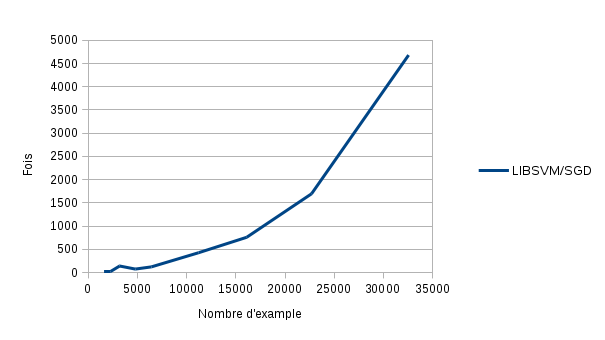
\includegraphics[width=120mm]{images/res}
\caption{Comparaison de la vitesse entre LIBSVM et SGD binaire}
\label{fig:res}
\end{figure}

\pagebreak
Par rapport au table \ref{tab:svmsgd}, nous trouvons que le taux de classification de SGD-SVM et SVM est presque pareil tandis que le temps d'apprendre est différent. La vitesse de SGD-SVM est très vite que la vitesse de SVM standard. Cet avantage de SGD-SVM est plus claire quand le nombre d'exemples d'apprentissage augmente. Cette chiffre est démontrée dans la colonne de table \ref{tab:svmsgd} ou aussi dans le figure \ref{fig:res}.\\

Les données que nous avons utilisé ont 123 caractéristiques. Nous trouvons que quand le nombre d'exemple est de 1,605, la méthode SGD est plus vitesse que la méthode SVM 10 fois, mais quand le nombre d'exemple de 32,561, SGD plus vitesse que SVM 4,682 fois. Ce chiffre confirme que la méthode SGD est beaucoup plus vitesse que SVM, surtout pour les grandes données. Donc, la méthode SGD s'adapte mieux au problème de classification d'image dont la base de données est très grande. En raison de son avantage, nous voulons la développer pour qu'elle puisse résoudre le problème de classification de multi-classes pour utiliser dans la domaine de classification d'images.


\section{Méthode MC-SGD}
Avant d'utiliser pour le problème de classification d'images, nous testons cette méthode avec les données multi-classes de LIBSVM \cite{svmdatamul}. Tout d'abord, on teste avec la base de données \textit{Protein} de 3 classes


\begin{table}[h]
\begin{center}
    \begin{tabular}{ | c | c | c | c | c | c | c |}
    \hline
    Données & LIBSVM(\%) & SGD(\%) & LIBSVM(s) & LIN(s) & PARAL(s) & $\frac{SVM(s)}{PARAL(s)}$ \\ \hline
    
    Protein & 68.23 & 68.66 & 511 & 0.35 & 0.2 & 2555 \\ \hline
    
    \end{tabular}
\end{center}
\caption{Comparaison entre LIBSVM et MC-SGD linaire et MC-SGD parallèle}
\label{tab:mcsvm}
\end{table}


En voyant le table \ref{tab:mcsvm}, nous trouvons que la méthode MC-SGD parallèle plus vite que la méthode SVM 2555 fois. Nous trouvons aussi que la version parallèle n'est pas beaucoup plus vite que sa version linaire. La raison est que le temps d'apprendre d'un classificateur est très petit et cette base de données ne comprend que 3 classes. Donc, La version parallèle économie seulement 0.15 seconds.\\

A fin de vous montrer la vitesse de la version parallèle de MC-SGD, nous avons testé avec la base de données de 10 classes\\

\begin{table}[h]
\begin{center}
    \begin{tabular}{ | c | c | c | c | c | c | c |}
    \hline
    Données & LIBSVM(\%) & SGD(\%) & LIBSVM(s) & LIN(s) & PARAL(s) & $\frac{SVM(s)}{PARAL(s)}$ \\ \hline
    
    mnist & 86.92 & 86.46 & 2810 & 0.86 & 0.72 & 3902.8 \\ \hline
    
    fr & 84.08 & 88.58 & 327 & 3.60 & 1.64 & 199.4 \\ \hline
    
    3d & 76.54 & 76.8 & 144 & 1.62 & 0.90 & 160 \\ \hline
    
    \end{tabular}
\end{center}
\caption{Comparaison entre LIBSVM et MC-SGD linaire et MC-SGD parallèle}
\label{tab:pmcsvm}
\end{table}


En générale, le résultat de classification de MC-SGD ne meilleure pas que SVM. Par contre, le temps d'apprendre est beaucoup plus vite que SVM pour le problème de classification de multi-classes. Le table \ref{tab:pmcsvm} est une preuve.

Cette expérimentation est déroulée dans l'ordinateur de 8 cœurs, la version parallèle n'est pas beaucoup plus vite que la version linaire car j'ai utilisé l'option d'optimiser le temps de toute les deux versions et le résultat de classification est le même. Donc, dès maintenant, les autres comparaisons entre SVM et MC-SGD seront réalisées avec la version parallèle.


\section{Classification d'images avec MC-SGD}
Comme nous avons parlé dans le processus, notre processus pour la classification d'images comprend 3 étapes principales : extraction des descripteurs avec le descripteur SIFT, construit la dictionnaire avec la méthode K-MOYENNE et l'apprentissage automatique pour la classification avec la méthode MC-SGD. Dans la partie précédente nous avons présenté le résultat de la méthode MC-SGD(l'étape 3, l'étape d'apprentissage automatique) avec la base de données existantes. Maintenant nous appliquons la méthode Sac de Mots pour préparer les entrées pour la méthode MC-SGD avec les bases d'images de classification pour voir si la méthode MC-SGD s'adapte pour le problème de classification d'images.


\begin{table}[h]
\begin{center}
    \begin{tabular}{ | c | c | c | c | c | c |}
    \hline
    Données & LIBSVM(\%) & SGD(\%) & LIBSVM(s) & SGD(s) & $\frac{SVM(s)}{SGD(s)}$ \\ \hline
    
    Scènes 8 catégories & 58.04 & 57.74 & 15 & 0.18 & 83.3 \\ \hline
    
    Caltech 101 & 61.52 & 67.12 & 2873 & 106.95 & 26.9 \\ \hline    
    
    Caltech 101 & 61.52 & 57.12 & 2873 & 74 & 38.8 \\ \hline   
    
    Caltech 7 3D & 91.52 & 88.3 & 113.4 & 0.81 & 140 \\ \hline    
    
    \end{tabular}
\end{center}
\caption{Comparaison entre LIBSVM et MC-SGD parallèle pour la classification d'images}
\label{tab:pmcsvm-8scenes}
\end{table}

Le tableau \ref{tab:pmcsvm-8scenes} montre que le pourcentage de classification de SVM est presque égale que MC-SGD. Par contre, SVM est plus lent que MC-SGD environs 20 fois, ça dépend la base de test. Ces bases d'images ne sont pas très grandes, la première ne contient que 8 catégories, la deuxième de 101 classes et la troisième de 7 classes. Nous rappelons que LIBSVM utilise one-vs-one et MC-SGD utilise one-vs-all. Donc, si la base d'image augmente plus de catégories ou classes, la méthode MC-SGD sera plus vitesse si on compare avec la méthode SVM.

%./svm-train -s 0 -c 312 -t 0 -g 0.0005 -e 0.1 data/scenes-8/scenes-libsvm.train 
%./sgdsvm -iter 1000 -k 10 -lambda 0.6 -paral 1 -testFile data/scenes-8/scenes-libsvm.test data/scenes-8/scenes-libsvm.train 


